\chapter{Zdroje dát pre analýzu}
\label{data-sources-available-for-research}

% # PART 2
% # TODO obsah by mal napovedat, ze vysledky boli dosiahnute
%        nejčastěji navštěvovaných stránek
%        Selenium
%        výhody a nevýhody vlastnych a externych dat
% # TODO sekcia o automatizovanom prehliadani stranok, Playwright
% # TODO nie je az tak dolezite, ze su najnavstevovanejsie, ako ze sa to automatizuje
% # TODO spomenut ale aj Selenium

Poznávacím znamením využívania technológie NEL je prítomnosť hlavičiek \code{NEL} a \code{Report-To} v HTTP odpovediach z monitorovaných web serverov. 
Pre účely analýzy jej využívania je teda nutné získať dáta obsahujúce tieto odpovede.
Cieľom je pozerať sa buď na reálne komunikácie, ktoré už prebehli, alebo skúmať ako web servery aktuálne dosiahnuteľné na internete
odpovedajú na HTTP požiadavky. 
V tejto kapitole sú detailne popísané dostupné zdroje dát a konkrétne spôsoby, akými možno záznamy takýchto komunikácií získať.

\section{Potrebné dáta}

V prvom rade je nutné definovať množinu webových serverov, pre ktoré možno získať potrebné záznamy HTTP komunikácie.
Vzhľadom na to, že web servery možno adresovať pomocou ich doménového mena, ďalej tieto web servery označujem ako skúmané domény.
Množinu skúmaných domén možno zaobstarať z niekoľkých zdrojov, ktoré sú popísané v sekcií \ref{tranco}.

Po definovaní množiny skúmaných domén je možné zmienené záznamy o komunikácií s nimi získať podľa toho, kedy komunikácia prebehla:
\begin{enumerate}
    \item Súčasnosť -- aktuálne dáta:
    
    Z hľadiska prítomnosti je možné použiť napríklad techniku automatizovaného webového prehliadania.
    Na účel toho je možné použiť už existujúce technológie ako Selenium alebo Playwright, ktoré opisuje sekcia \ref{selenium}.

    \item Minulosť -- historické dáta:

    Pre sledovanie historického vývoja nasadenia NEL je tiež nevyhnutné nahliadnuť do histórie prevádzky skúmaných domén. 
    Z tohto hľadiska je nutné použiť už spracované a uložené dáta. 
    Vyhovujúcim zdrojom historických dát je napríklad projekt \textbf{HTTP Archive}, ktorému sa táto práca venuje primárne, a to v sekcií \ref{httparchive}.
    Ide o službu, ktorá zaznamenáva vývoj webu od roku 2010 a teda jej vhodnosť sa potvrdzuje tým, že špecifikácia NEL v tejto práci bola publikovaná až v roku 2018.
\end{enumerate}

\pagebreak

\section{Množina skúmaných domén}
\label{tranco}

% Platí, že čím je mohutnejšia množina skúmaných domén, tým presnejšiu analýzu využívania NEL na webe možno vypracovať.
% Preto je pri výbere takejto množiny kľúčová jej mohutnosť.
Existujú projekty, ktoré sa zaoberajú získavaním doménových mien pre rôzne účely.
Niektoré sú vypracované na to aby uchovávali tie, ktorých webstránky sú najčastejšie navšetevované \cite{hacker-target-website-lists-overview, tranco}.
Iné projekty zase spravujú zoznam tých, ktoré navštevujú používatelia iných služieb autorov daného projektu \cite{chrome-crux}. 

\subsection{Najčastejšie navštevované domény}

Jeden z projektov, ktorých účelom je zaznamenávanie domén s najčastejšie navštevovanými webstránkami je TRANCO \cite{tranco}.
Projekt TRANCO poskytuje sadu nástrojov pre generovanie rebríčkov najpopulárnejších domén. 
Tieto rebríčky webových domén zoradených podľa hodnotenia návštevnosti ich webstránok je odolný proti externej manipulácií a vhodný na účely výskumu. 
Vznikol na základe častej potreby pre skúmanie práve takýchto domén či už pre jednoduchú referenciu, alebo ako podklad pre ďalší prieskum.
TRANCO nie je prvým takýmto rebríčkom, ale je prvým, ktorý sa zaoberá nedostatkami iných existujúcich rebríčkov.
Existujúce rebríčky využíva ako zdroje dát pre tvorbu toho svojho.
Nový rebríček TRANCO sa tvorí zlučovaním zdrojových rebríčkov do nového, stabilnejšieho rebríčka, ktorý reprezentuje domény v globálnej škále.
TRANCO dokonca do určitej miery odstraňuje zo zdrojových rebríčkov domény, na ktorých môže byť zverejnený nežiadúci (nebezpečný) obsah.
Obsahuje primárne registrovateľné domény, čo sú domény, ktoré si môže priamo zakúpiť či už jednotlivec alebo organizácia. 
Príkladom môžu byť domény registrované pod TLD \code{com}, ale aj domény registrované pod eTLD zo zoznamu verejných suffixov ako \mbox{\code{co.uk} \cite{tranco}}.

TRANCO je podložený štúdiom zameraným na vylepšenie dostupných alternatív rebríčkov populárnych domén.
Práve tieto alternatívne rebríčky tvoria vnútorne použité zdroje dát pre výsledné rebríčky TRANCO.
Medzi ne patria projekty \cite{tranco-config}:
\begin{itemize}
    \item Alexa Top Sites,
    \item Majestic Million,
    \item Cisco Umbrella,
    \item Quantcast,
    \item Chrome User Experience Report,
    \item Cloudflare Radar.
\end{itemize}
TRANCO je ako zdroj skúmaných domén pre túto prácu vhodný, pretože sprístupňuje a vylepšuje presnosť záznamov z týchto alternatív.
Taktiež udržiava ich historické dáta, ktoré už nie sú samostatne dostupné.
Vzhľadom na to je možné preskočiť výber toho najvhodnejšieho z pomedzi nich a použiť práve TRANCO.

\subsection{Generovanie rebríčka TRANCO}
\label{tranco-generation}

V jeho štandardnej forme, rebríček TRANCO sa generuje každý deň v dvoch verziách:
\begin{itemize}
    \item TRANCO rebríček domén
    \item TRANCO rebríček domén a subdomén
\end{itemize}

V tomto každodenne generovanom rebríčku sú prednastavené aj zdroje dát, teda použité zdrojové rebríčky, aj dátumový rozsah, za ktorý sa zo zdrojových rebríčkov má čerpať.
Štandardne sa vytvára výsledok z rebríčkov Chrome User Experience Report, Majestic Million, Cloudflare Radar a Cisco Umbrella.
Dátumový rozsah je nastavený na posledných 30 dní \cite{tranco-config}, pričom TRANCO použije ako kompletný zdroj dát všetky spomenuté rebríčky vygenerované za túto dobu. 

V novom TRANCO rebríčku sa zo zdrojových rebríčkov spriemeruje pre každú doménu jej zaradenie aplikovaním jednej z dostupných kombinačných metód pre upravenie finálneho hodnotenia domén.
Pre štandardný rebríček je využitá kombinačná metóda takzvanej harmonickej progresie, nazývaná Dowdall rule. 
Dowdall rule hodnotí v zozname obsahujúcom N domén prvú hodnotou 1 a všetky ostatné postupne \(1/2\), \(1/3\) až \(1/(N-1)\) a zakončí hodnotením poslednej -- \(1/N\) \cite{tranco, tranco-config}.
Názornú ukážku aplikovania Dowdall rule na rebríčky vizualizuje obrázok \ref{img:dowdall-rule}.
Generuje sa v ňom nový rebríček o veľkosti štyroch domén, takže sa do úvahy beriú prvé štyri domény z každého vstupného rebríčka. 
Skóre sa vypočíta podľa umiestnenia a podľa celkového počtu domén radených v danom zdrojovom rebríčku. 
Rebríček 4 (v obrázku úplne napravo) s najvyšším počtom hodnotených domén výsledok ovplyvnil najviac.

\begin{figure}[htb]
\begin{center}
 % 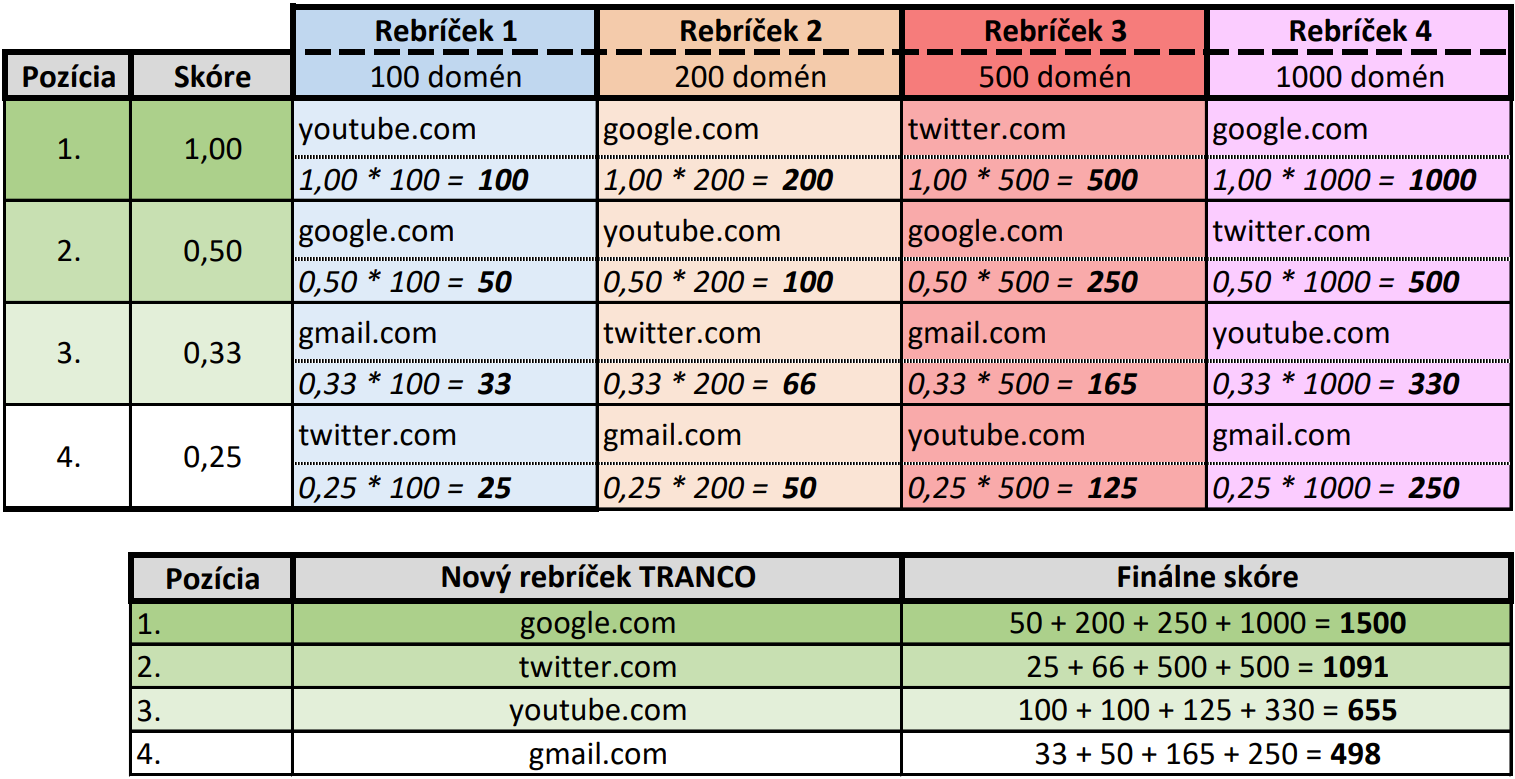
\includegraphics[scale=0.375]{obrazky-figures/dowdall_rule.png}
 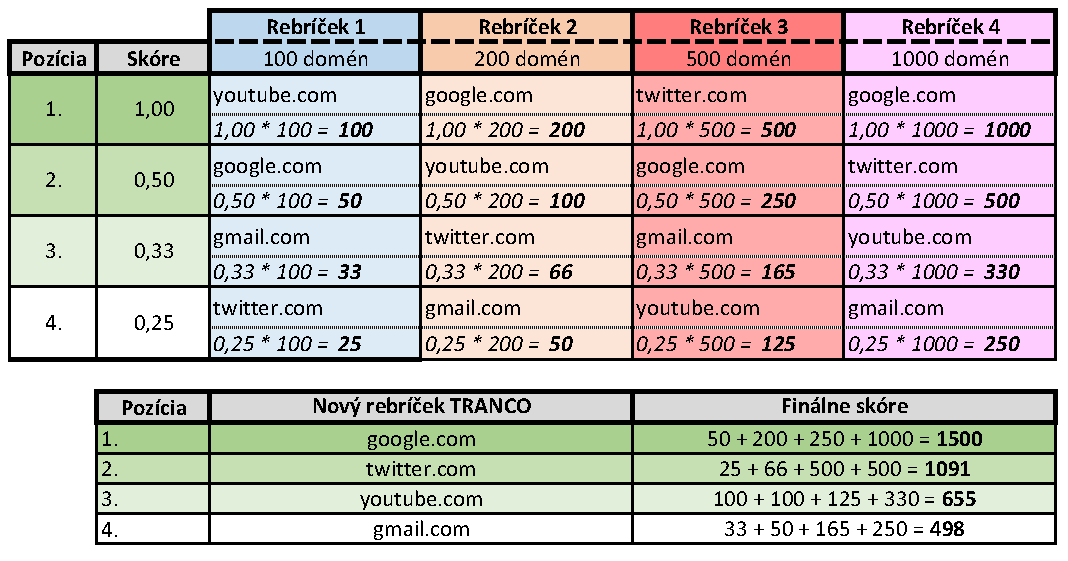
\includegraphics[scale=0.84]{obrazky-figures/dowdall_rule_size_fit_cropped.pdf}
 \caption{\centering Príklad uplatnenia Dowdall rule na spriemerovanie štyroch vstupných rebríčkov do výsledného rebríčka TRANCO.}
 \label{img:dowdall-rule}
\end{center}
\end{figure}

Po dokončení priemerovania a zoraďovania sa spolu s výsledným rebríčkom vytvorí na oficiálnom webe TRANCO aj jedinečná stránka obsahujúca odkaz na jeho stiahnutie a tiež citácia, 
ktorou je možné jedinečne odkazovať na tento nový rebríček v prácach, ktoré ho môžu použiť na svoje účely.
Zároveň, okrem generovania nových TRANCO rebríčkov sú na oficiálnej stránke dostupné aj historicky vygenerované, spomenuté štandardné, každodenné rebríčky \cite{tranco-homepage}.

Príklad obsahu vygenerovaného rebríčka znázorňuje výpis \ref{listing:tranco-obsah}.
Rebríček je možné stiahnuť vo formáte \code{zip} archívu, ktorý obsahuje práve jeden súbor nazvaný \textbf{top-1m.csv}. 
Obsahom je na každom riadku čiarkou oddelené umiestnenie domény a jej meno.

\pagebreak

\begin{center}
\centering
\begin{lstlisting}[
caption={\centering Ukážka vygenerovaného denného rebríčku z 12. januára 2024, orezaného na prvých 10 domén.},
label=listing:tranco-obsah, 
language=json, 
frame=lb,
xleftmargin=.3875\textwidth, 
xrightmargin=.3875\textwidth]
1,google.com
2,amazonaws.com
3,facebook.com
4,microsoft.com
5,a-msedge.net
6,googleapis.com
7,apple.com
8,youtube.com
9,akamaiedge.net
10,akamai.net

\end{lstlisting}
\end{center}


\section{Automatizované prehliadanie webu}
\label{selenium}

Táto sekcia ešte nie je napísaná.

\section{HTTP Archive}
\label{httparchive}

Projekt HTTP Archive sa zaoberá zaznamenávaním spôsobu konštrukcie a poskytovania digitálneho obsahu na webe. Je permanentným repozitárom informácií o webe a udržiava záznamy ako veľkosti
stránok, zlyhané HTTP požiadavky alebo technológie využité v rámci konkrétnej stránky. Vďaka týmto dátam je možné pozorovať trendy v histórií vývoja webu ako celku a zároveň je nad nimi možné vykonávať
rôzne podrobné prieskumy a analýzy \cite{httparchive-about}. 

Autormi HTTP Archive sú členovia komunity zvanej Web Performance Group. Pôvodným autorom je Steve Souders, ktorý projekt založil v roku 2010 \cite{httparchive-faq}.
Momentálne sa na jeho údržbe po stránke vývoja podieľa štvorica hlavných členov, a keďže ide o open source projekt, v prevádzke ho udržiavajú sponzori ako aj spoločnosti Google, Mozilla, O'Reilly Media a Fastly.
Taktiež je tento projekt súčasťou projektu Internet Archive, ktorý už od roku 1996 slúži ako digitálna knižnica poskytujúca zadarmo prístup ku knihám, filmom, hudbe a rovnako aj k miliardám archivovaných webstránok \cite{httparchive-about}.

Cieľom projektu je vytvoriť a udržiavať služby poskytujúce možnosť nahliadnuť do minulosti webu, pozorovať jeho prechod do momentálneho stavu a vďaka získaným náhľadom a poznatkom dokázať
predpovedať potencionálne nové trendy blízkej budúcnosti. 
Pre tento účel vyvinuli sadu nástrojov pre zbieranie uvedených dát z verejného internetu, efektívne ukladanie nadobudnutých dát a ich reprezentáciu na svojom webe.
Naviac sa na uskladnenie dát používa služba \textbf{Google Cloud Platform (GCP)}.
Tieto dáta sú v rámci GCP verejne prístupné ako databázové tabuľky v prostredí GCP zvanom \textbf{BigQuery}, čo zastrešuje aj potrebu pre prostredie na prehliadanie dát pomocou SQL príkazov 
a vykonávanie komplexných analýz nad dátami HTTP Archive \cite{httparchive-faq}. 

\pagebreak

Vhodnosť projektu pre túto prácu je založená na tom, že ide o komunitný projekt, ktorého výsledky sú verejne a zadarmo dostupné. Keďže umožňuje prístup k historickým záznamom reálneho prenosu HTTP(S) komunikácie na webe, ktoré siahajú až po rok 2010, prirodzene sa z neho stáva primárny zdroj pre výskumy a analýzy, akou je aj analýza v rámci tejto práce.


\subsection{Získavanie dát}
\label{fetching-data}

Základom pre všetky činnosti HTTP Archive sú dáta o stave webu. Tie sú získané pravidelným spúšťaním procesu zvaného \textbf{Web Crawling}.
Web Crawling je technika skúmania webu, ktorá programovo vstúpi na zvolenú stránku a získava o nej informácie ako metadáta, jej obsah a iné dáta v oblasti záujmu \cite{httparchive-webcrawling}.
HTTP Archive pomocou web crawlingu získava dáta ohľadom celkového aplikačného prenosu, kde meranou dátovou jednotkou je žiadosť, teda HTTP \textbf{request}, a odpoveď, teda HTTP \textbf{response}, ktorou web server zareaguje. 
Keďže môžu nastať odlišnosti v komunikácií vedenej z bežného počítača oproti takej, ktorá je vedená z mobilného zariadenia, HTTP Archive zaznamenáva výsledky aj z \textbf{desktop}, aj z \textbf{mobilného} prostredia.
Zo získaných dát potom svojimi algoritmami extrahuje všetky dôležité poznatky, medzi ktoré patria napríklad aj stránkou používané zdroje a použité webové aplikačné rozhrania (Web API) \cite{httparchive-homepage}.

Výber vstupov do tohto procesu predstavuje hľadanie vhodnej sady záznamov URL na skúmanie. 
HTTP Archive na to momentálne používa projekt \textbf{Chrome User Experience Report}, spomínaný už v sekcii \ref{tranco-source-rankings}.

\subsubsection{WebPageTest}

Získané URL adresy sú použité ako vstup do programu WebPageTest. WebPageTest (ďalej označovaný už iba ako WPT) je softvér na testovanie výkonnosti webových stránok vyrobený spoločnosťou Google. 
Predstavuje komplexné riešenie schopné testovať a merať proces načítavania, vykresľovania a využitia siete pre vybrané web stránky. 
Je zverejnený priamo na stránkach jeho oficiálneho repozitára GitHub\footnote{\href{https://github.com/catchpoint/WebPageTest}{https://github.com/catchpoint/WebPageTest}} spolu s priloženou dokumentáciou, a to pod open source licenciou.
Medzi konkrétne skúmané metriky patria napríklad: \cite{webpagetest}
\begin{itemize}
    \item Time to First Byte (TTFB) --- čas do prvej časti odpovede od servera
    \item First Contentful Paint (FCP) --- čas do začiatku načítavania obrázkov a grafiky
    \item Largest Contentful Paint (LCP) --- čas do načítania najväčšej časti obsahu stránky 
    \item Cumulative Layout Shitf (CLS) --- posun a zmena rozpoloženia obsahu stránky počas jej načítavania
\end{itemize}

HTTP Archive na svoje účely používa vlastnú WPT inštanciu. 
Táto inštancia je priebežne synchronizovaná s najnovšou dostupnou verziou.
Vo svojich behoch využíva užitočnú funkcionalitu WPT --- vlastné (prispôsobené) metriky.
Pridanie vlastných metrík do WPT predstavuje spúšťanie hocijakej funkcie spísanej v jazyku JavaScript na konci behu testovania stránky. 
Využívaním tohto dokáže HTTP Archive zbierať akékoľvek dodatočné metriky zo svojich testovacích stránok \cite{webpagetest}.

\pagebreak

Je dôležité poznamenať, že stránky sú testované s čistou vyrovnávacou pamäťou cache. 
Taktiež sa na stránkach vyžadujúcich autentifikáciu nikdy neprihlasuje.
To môže spôsobovať odchýlku oproti reálnemu používaniu testovacích web stránok. 
Ďalšou limitáciou je fakt, že každá stránka je preskúmaná samostatne a neberie sa žiaden ohľad na jej podstránky.
WPT je spúšťaný vždy prvý deň v mesiaci a teda obsahuje dáta užitočné za posledný mesiac, kde môže ale nastať duplicita dát v prípade, že predošlý beh WPT trval výrazne dlho.

Pre účely uskladňovania získaných dát je využitý formát HTTP Archive súboru (prípona \code{.har}, ďalej označovaný už len ako HAR).
Formát HAR je prispôsobený na uskladňovanie dát spojenia nadviazanom vo webovom prehliadači. Samotné dáta sú serializované ako JSON - JavaScript Object Notation.
Bežným obsahom HAR súboru býva HTTP žiadosť, prislúchajúca odpoveď, metriky výkonnosti načítania stránky a iné \cite{httparchive-harfile}. 
Orientačný príklad obsahu takéhoto súboru je ukazuje výpis \ref{listing:harfile}.

\begin{center}
\centering
\begin{lstlisting}[caption={\centering Orientačná ukážka obsahu súboru HAR. Všetky detaily o získaní zdroja z web servera je zaznamenaný v položke \code{"log"}. Hlavná štruktúra tejto položky je zložená z párov kľúč--hodnota, kde \code{"version"} definuje verziu súboru HAR , \code{pages} obsahuje napríklad URL získaného zdroja a \code{entries} obsahuje HTTP žiadosť \mbox{a odpoveď pre daný zdroj.}},
label=listing:harfile, 
language=json, 
frame=tb,
xleftmargin=.09\textwidth, 
xrightmargin=.09\textwidth]
{
  "log": {
    "version": "1.2",
    ...
    "pages": [
      {
        "startedDateTime": "2024-01-12T15:25:01.278Z",
        "id": "page_1",
        "title": "https://tranco-list.eu/list/KJ49W/1000000",
        "pageTimings": {...}
      }
    ],
    "entries": [
      {
        ...
        "request": {...},
        "response": {...},
        ...
      },
      ...
    ]
  }
}
\end{lstlisting}
\end{center}


Úspešne serializované a vhodne formátované dáta sú po skončení behu WPT nahrané do existujúcich databázových tabuliek na GCP, čím sú sprístupnené pre používanie \cite{httparchive-faq}. 

\subsection{Skladovanie a práca s dátami}
Google Cloud Platform (GCP) je súčasťou balíčka služieb Google Cloud. 
Výraz \textbf{cloud} sa používa pre množinu serverov používaných napríklad na výpočtové práce alebo skladovanie dát, ktoré sú prepojené cez internet.
Tieto servery zostavujúce cloud infraštruktúru môžu poskytovať rôzne programové riešenia, ktoré sa v terminológii spojenej s cloud výpočtami nazývajú služby \cite{cloudflare-clouddefinition}.

Súčasťou infraštruktúry patriacej práve Google je už spomínaný GCP. Predstavuje výpočtové služby združené pod záštitu jednotnej platformy.
Tieto služby sú rozdelené do kategórií ako výpočtová sila, ukladací priestor, sieťové riešenia, dátová analýza a strojové učenie \cite{gfg-gcp}.
Časť záujmu tejto práce spadá práve do kategórie ukladacieho priestoru, kam sa radí služba \textbf{BigQuery}.

\subsubsection{GCP BigQuery}
\label{big-query}

BigQuery, infraštruktúra pre ukladanie dát v rámci GCP, je produkt, ktorý umožňuje jeho užívateľom spravovať a analyzovať dáta za pomoci vstavaných funkcionalít ako napríklad aj strojového učenia.
BigQuery je samo o sebe riešenie populárne označované ako \textbf{platforma poskytovaná ako služba} (PaaS).
Hlavnou výhodou pre užívateľov služby typu PaaS je, že sa nemusia nijako starať o správu infraštruktúry, pod čím sa vlastne myslí daná platforma, kde je služba sprevádzkovaná.
O správu potrebnej infraštruktúry (servery, sieťové prvky, bezpečnosť) sa stará GCP, teda poskytovateľ tejto služby.
Tým pádom je možné BigQuery ako skladisko dát veľmi rýchlo zakomponovať do akéhokoľvek vlastného projektu \cite{google-bq}.

Dôležitou vlastnosťou Big Query je prispôsobenosť na vysokorýchlostné výpočty nad obrovským množstvom dát.
Distribúcia výpočtov umožňuje docieliť vykonávanie analýzy nad dátami o veľkosti v terabajtoch za sekundy (TB/s) a petabajtoch za minúty (PB/m).
K tomu napomáha špeciálna vnútorná reprezentácia uložených tabuliek. 
Bežný spôsob ukladania dát do tabuliek v databáze je takzvaný riadkovo orientovaný.
Orientovanie na riadky znamená, že sa záznamy v tabuľke ukladajú priamo vedľa seba na disk databázy.
To je vhodné pre prípady, keď majú byť na úložisku záznamy hľadané individuálne.
Avšak, pre zložité analytické výpočty nad veľkým objemom dát to predstavuje problém vo výkonnosti, pretože sa musia potupne pre každý záznam tabuľky prehľadať všetky jeho polia \mbox{(stĺpce) \cite{google-bq}}.

\begin{figure}[htb]
\begin{center}
 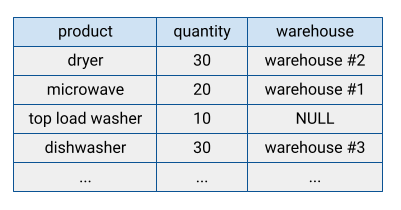
\includegraphics[scale=0.7]{obrazky-figures/row-oriented-store.png}
 \caption{\centering Príklad uskladnenia dát v riadkovo orientovanej databáze. Prechádzať dáta po riadkoch predstavuje musieť prehľadať všetky jeho stĺpce.}
 \label{img:row-oriented-store}
\end{center}
\end{figure}


Riešenie, ktorým BigQuery tento problém adresuje je použitie orientácie na jednotlivé stĺpce. 
Ukladaním dát v stĺpcovom formáte, a teda ukladaním každého stĺpca separátne umožňuje prehľadávať dataset bez viazania sa na všetky ostatné stĺpce.
Tým sa efektívne znižuje množstvo dát, ktoré sa prehľadávajú naraz.
Takto je databáza optimalizovaná pre analýzy nad obrovským množstvom uložených záznamov \cite{google-bq}.

\begin{figure}[htb]
\begin{center}
 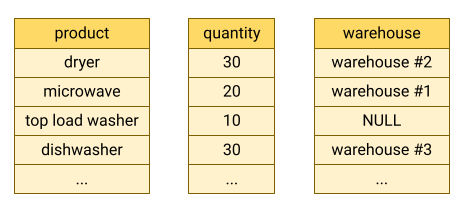
\includegraphics[scale=0.7]{obrazky-figures/column-oriented-store.png}
 \caption{\centering Príklad uskladnenia dát s využitím orientácie na jednotlivé stĺpce. Dáta je takto možné prehľadávať rýchlejšie a efektívnejšie, pričom sa spracuje menší objem dát. To vyhovuje používateľom BigQuery, ktorí sú obmedzení dostupným objemom dát \mbox{(viď platobné plány BigQuery na konci tejto sekcie).}}
 \label{img:column-oriented-store}
\end{center}
\end{figure}

Dáta skladované v BigQuery sú organizované do skupín klasických databázových tabuliek nazývaných \textbf{dataset}.
Na GCP je dostupné množstvo datasetov pre prehľadávanie.
Je nutné si najprv založiť \textbf{Google Cloud projekt} na oficiálnej stránke, ktorý slúži ako menný priestor pre zdroje, ktoré užívateľ do neho pridáva a používa.
K dátam je možné priamo pristupovať prostredníctvom troch rozhraní: \cite{google-cloud} 
\begin{enumerate}
    \item Google Cloud Console

    Webové grafické rozhranie pre spravovanie Google Cloud projektov. 
    Časť Google Cloud Console, ktorú užívatelia môžu využiť špecificky na prehliadanie dát BigQuery sa nazýva \textbf{BigQuery Studio}.
    Výhodou tohto spôsobu pracovania so zdrojmi je vysoká úroveň interaktivity, ktorú ponúka zabudované integrované vývojové prostredie pre prácu s dátami. 
    
    \item BigQuery nástroj príkazového riadku

    Pre zobrazovanie databáz a tabuliek, prehľadávanie a spravovanie dát v prostredí príkazového riadka je možné využiť nástroj s názvom \textbf{\code{bq}}. 
    
    \item BigQuery klientske knižnice

    Vďaka klientským knižniciam implementujúcim komunikačné rozhranie s BigQuery je taktiež dostupná možnosť programovo manipulovať a prehliadať zdroje priradené k užívateľskému projektu.
    Táto možnosť je vhodná pre predom definované, opakované úlohy, ktoré či už požadujú zdroje na vstupe, alebo ich počas svojho behu nahrávajú, prípadne upravujú podľa potreby.
\end{enumerate}

\pagebreak

Pri využití ktorejkoľvek z týchto možností platí, že prehliadanie a manipuláciu dát umožňuje jazyk SQL (Structured Query Language).
Ide o zaužívaný štruktúrovaný jazyk pre správu dát uložených v databáze.
V prostredí BigQuery sa používa dialekt pre SQL nazývaný \textbf{GoogleSQL}\footnote{\href{https://cloud.google.com/bigquery/docs/reference/standard-sql/query-syntax}{https://cloud.google.com/bigquery/docs/reference/standard-sql/query-syntax}} \cite{google-bq}.

Ako už bolo uvedené, HTTP Archive ukladá svoje výstupné dáta práve do Google Cloud.
Tieto dáta sa nachádzajú práve v Google Cloud Console dostupné ako \textbf{zdroj} (anglicky resource), ktorý si môže prihlásený používateľ pridať do svojho projektu.
Po pridaní tohto zdroja s priradeným názvom \code{httparchive} do projektu\footnote{\href{https://github.com/HTTPArchive/httparchive.org/blob/main/docs/gettingstarted\_bigquery.md}{https://github.com/HTTPArchive/httparchive.org/blob/main/docs/gettingstarted\textunderscore bigquery.md}} sa sprístupnia pre používanie nasledovné datasety: \cite{httparchive-repo}

\begin{itemize}
    \item \code{summary\_pages}:

    Obsahuje detaily o jednotlivých web stránkach ako časy ich načítania, počet žiadostí o jej zdroje, typy zdrojov a ich veľkosti.
    Taktiež sú tu informácie týkajúce sa presmerovaní, vzniknutých chýb, použitých služieb ako CDN\footnote{\href{https://www.cloudflare.com/learning/cdn/what-is-a-cdn/}{https://www.cloudflare.com/learning/cdn/what-is-a-cdn/}} a iné.
    
    \item \code{summary\_requests}:

    Nachádzajú sa tu dáta o konkrétnych objektoch načítaných ako už spomínané zdroje pre web stránky v datasete \code{summary\_pages}.
    V dátach je možné prehľadávať ako boli zdroje načítané priamo v hlavičkách HTTP odpovede, v ktorej prišli zo serveru poskytujúceho danú stránku.
    
    \item \code{pages}:

    Extrahované HAR súbory pre každú URL z prehľadávaných web stránok.
    
    \item \code{requests}:

    Extrahované HAR súbory pre každý zdroj jednotlivých prehľadávaných web sránok \mbox{v \code{pages} datasete}.
    
    \item \code{response\_bodies}:

    Extrahované HAR súbory obsahujúce celé telo HTTP odpovede z každej URL prehľadávaných web stránok.
    Ide o veľmi veľké tabuľky, ktoré môžu dosahovať veľkosť \mbox{v jednotkách terabajtov (TB)}.
\end{itemize}

BigQuery zdroj \code{httparchive} sprístupňuje aj niekoľko ďalších datasetov, no práve tie spomenuté vyššie tvoria sadu dôležitých, ktorými sa táto práca zaoberá. 

Každý z týchto datasetov obsahuje tabuľky nazvané podľa rovnakej konvencie --- dátum vykonaného zberu dát a prostredie, v akom prebiehal.
Dátum je definovaný formátom YYYY\_MM\_DD, kde YYYY predstavuje rok, MM mesiac a DD deň. Prostredie môže byť buď počítačové alebo mobilné, ako sa spomína už v sekcii \ref{fetching-data}.
Príkladom názvu tabuľky teda môže byť '\code{2023\_01\_01\_mobile}' alebo '\code{2023\_01\_01\_desktop}'.

\pagebreak

\begin{figure}[htb]
\begin{center}
 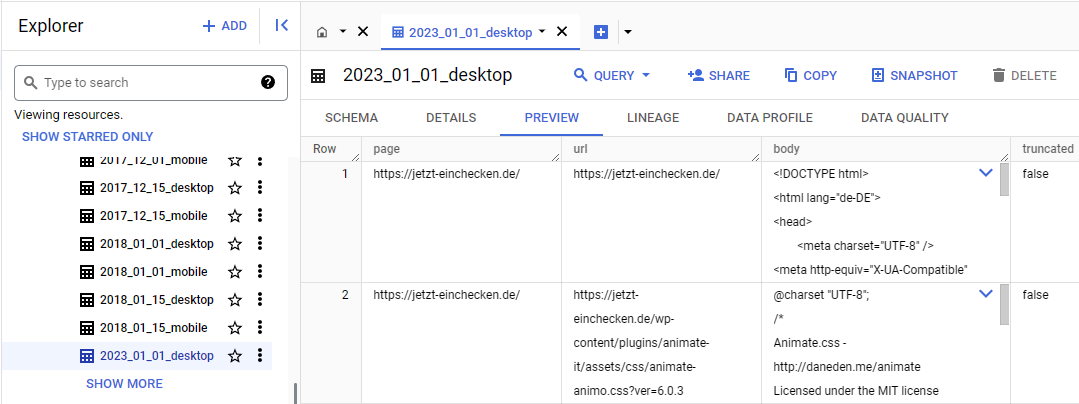
\includegraphics[scale=0.53]{obrazky-figures/bigquery_response_bodies.png}    
 \caption{\centering Otvorené okno v GCP BigQuery pri pohľade na otvorený prehľad datasetu '\code{2023\_01\_01\_mobile}'. 
 Jednotlivé uložené položky sú: \code{page}, \code{url}, \code{body} a \code{truncated}.}
 \label{img:bigquery-example-table}
\end{center}
\end{figure}


Za použitia GoogleSQL je možné datasety kombinovať a vytvárať komplexné sady dát (ako na obrázku \ref{img:bigquery-example-query}) pre ďalšiu analýzu.
Prehľadávaním týchto dát a sledovaním HTTP hlavičiek je možné dopracovať sa k HTTP odpovediam, ktoré obsahujú hlavičky (pravidlá) technológie NEL.
Každú doménu, ktorá vo svojich odpovediach zaslala hlavičku NEL, môžem skúmať ako doménu s nasadeným monitorovaním NEL.

\begin{figure}[!htb]
\begin{center}
% height=8.401cm
 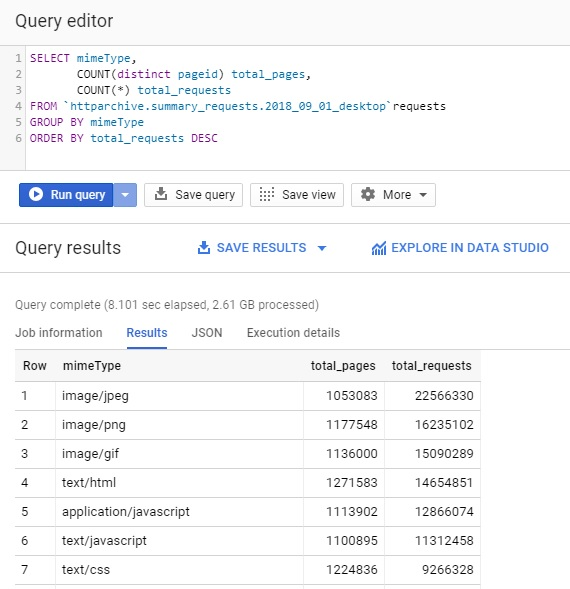
\includegraphics[width=11cm, height=10.0125cm]{obrazky-figures/mimeType_summary_example_query.jpg}    
 \caption{\centering Ukážka vytvorenia vlastnej sady dát v prostredí GCP BigQuery. Za použitia príkazov GoogleSQL sú dáta transformované na zoznam typov MIME podľa ich využitia na stránkach uvedených v dátach.}
 \label{img:bigquery-example-query}
\end{center}
\end{figure}

\pagebreak

Čo sa platieb týka, GCP BigQuery pre užívateľov poskytuje bezplatný plán s nastavenými limitmi pre využívanie konkrétnych funkcií.
\textbf{Bezplatný plán} zahŕňa 1TB procesnej kapacity dát a 10GB úložného priestoru pre vlastné dáta, pričom dochádza každý mesiac \mbox{k obnove týchto bezplatných zdrojov}.
Po prečerpaní kapacity uvedenej v tomto pláne je nutné akékoľvek ďalšie operácie doplatiť.
Zoznam spôsobov, akými je možné zaplatiť za navýšenie spomenutých kapacít je rozsiahly, no pre prípady použitia tejto práce je relevantný platobný plán zvaný On-demand.
\textbf{On-demand plán}, alebo platba podľa potreby sa vzťahuje na procesnú kapacitu, ktorá sa vyčerpáva vykonávaním operácií nad dátami.
Cena za 1TB kapacity je v čase písania práce \$6.25, pričom stále platí, že prvý terabajt je každý mesiac zadarmo \cite{google-bq-pricing}.

% \subsection{Pravidelné správy o stave webu}

% Okrem samotných dát a prostredia na ich prehľadávanie zostavuje HTTP Archive projekt aj prehľady stavu webu formou interaktívnych grafov reprezentujúcich konkrétnu metriku v oblasti záujmu HTTP Archive.

% \subsubsection{Elementárne reporty metrík}
% Medzi takéto prehľady patrí napríklad report o zmene priemernej celkovej veľkosti konkrétnej načítanej stránky v kilobajtoch, alebo, taktiež relevantný je aj report zobrazujúci dosiahnuteľnosť HTTP Archive -- počet jedinečných URL analyzovaných týmto projektom (viď obrázok \ref{img:total-urls-report}).

% \begin{figure}[!htb]
% \begin{center}
%  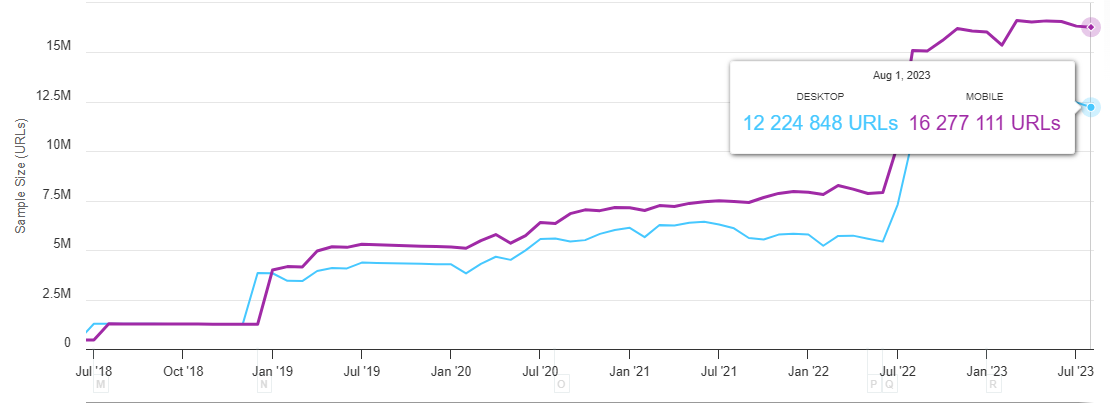
\includegraphics[scale=0.51815]{obrazky-figures/total_urls_report.png}    
%  \caption{\centering Report zobrazujúci počet URL adries analyzovaných v rámci projektu HTTP Archive. Graf reportu znázorňuje dáta od dátumu prvého web crawlingu vykonaného v rámci projektu. Momentálny počet URL adries zakomponovaných do datasetov v BigQuery je 12 224 848 pre testy vykonávané na počítači a 16 277 111 pre testy vykonávané zo simulovaného mobilného prostredia.}
%  \label{img:total-urls-report}
% \end{center}
% \end{figure}

% \pagebreak

% \subsubsection{Web Almanac}
% \label{web-almanac}
% Na takýchto a mnoho ďalších nízko úrovňových reportoch každoročne stavia aj komplexný report s názvom \textbf{Web Almanac}, ktorý tiež patrí pod túto iniciatívu.
% Web Almanac spája elementárne dáta do kontextualizovaných náhľadov, ktoré približujú jeho čitateľom stav webu na vysokej úrovni \cite{httparchive-methodology}.
% Posledný report bol už štvrtým vydaním v poradí.
% Vďaka skúsenostiam z predošlých troch rokov autori navýšili relevantnosti metrík, ktoré zahŕňa. 
% Všetky tieto skúmané metriky sú zároveň dostupné na GitHub stránkach projektu, kde každú jednu reprezentuje hotový SQL skript spustiteľný priamo v prostredí GCP Big Query.

% Celý obsah reportu je dostupný na jeho oficiálnej stránke\footnote{\href{https://almanac.httparchive.org/en/2022/table-of-contents}{https://almanac.httparchive.org/en/2022/table-of-contents}}. 
% Každý aspekt jeho prieskumu je zatriedený do svojej vlastnej kategórie, ktorá sa v rámci obsahu označuje ako samostatná kapitola.
% Čitatelia tu môžu nájsť napríklad kapitolu zameranú špecificky na JavaScript, použitie WebAssembly na webe, ale aj pre túto prácu relevantnejšie oblasti ako HTTP a bezpečnosť.

% Celkovo sa snahou viacej ako 100 prispievateľov podarilo takouto formou štruktúrovane zaznamenať stav webu textovo, ale aj pomocou detailných grafových vizualizácií.
% Autori sa snažia zvýšiť rozsah projektu a tým aj počet sledovaných relevantných oblastí tak, že každý rok povzbudzujú nových potencionálnych prispievateľov do pripojenia sa k ich iniciatíve. 

% Do budúcna sa bude kvalita Web Almanac reportov zlepšovať. 
% V tohtoročnom reporte bude oproti tomu minuloročnému zahrnutých viac ako dvojnásobok vzoriek URL, 
% ktoré HTTP Archive podrobí svojmu web crawlingu.
% V ideálnom prípade to znamená, že sa dosah podkladov pre report efektívne zdvojnásobí a tým pádom má potenciál byť presnejší a globálne reprezentatívnejší.

% Využitie práve tohto reportu by bolo ideálnym spôsobom, ako \textbf{dostať technológiu NEL a jej využitie do verejného povedomia}. 
% Spoluprácou s autormi Web Almanac by sa jedna z nových kapitol budúcich vydaní mohla zaoberať technológiou NEL.

% \section{Alternatívy}
% \label{httparchive-alternatives}

% Aj keď je HTTP Archive najvhodnejším zdrojom dát pre účely tejto práce, existujú aj iné, ktoré stoja za zmienku.
% Dáta, ku ktorým máme prístup vďaka tomuto primárnemu zdroju síce sú postačujúce pre rôzne typy analýz. Sú ale dostupné aj zdroje disponujúce špecifickými výhodami, ktoré
% zase umožňujú či už spätne kontrolovať správnosť dát HTTP Archive, alebo na ne nadviazať.
% Z toho dôvodu sú niektoré alternatívy popísané v tejto kapitole.

% \subsection{crawler.ninja}

% Projekt \textbf{crawler.ninja} založený autorom Scottom Helme slúži ako podklad pre jeho prieskum
% webu, v ktorom pozoruje stav bezpečnosti na internete. 
% Výsledky tohto prieskumu autor prvýkrát zverejnil už v roku 2015, no o vytvorení projektu crawler.ninja na svojom blogu píše až v júli 2018 \cite{crawler-ninja}. 

% % \pagebreak

% Úmyslom autora pozorovať bezpečnosť vyúsťuje do jeho periodických reportov týkajúcich sa tejto tématiky. 
% Samotný projekt sa stará o zber dát pre zhotovenie týchto reportov.
% Aj keď zbieranie dát pretrváva do súčasnosti, posledný report od autora bol publikovaný dávnejšie --- 09.12.2021, od kedy zanechal svoju pravidelnosť (aspoň jeden report za rok).

% Crawler.ninja slúži na prehľadávanie webu technikou Web Crawling za cieľom získať dáta o web stránkach, ktoré autor plánuje skúmať.
% Ako vstup do tohto procesu, a teda zoznam použitých URL, sa používa rebríček populárnych stránok Alexa Top 1 milion.

% Crawl sa spúšťa každý deň a získané dáta ukladá (podľa toho čo autor zmieňuje na svojom blogu) do databázy MySQL, z ktorej je následne vytvorený takzvaný databázový export.
% Databázový export predstavuje súbor SQL príkazov, spustením ktorých môže ktokoľvek replikovať pôvodnú databázu aj s obsahom jej tabuliek. 
% Možnosť vytvoriť takýto súbor poskytuje priamo MySQL databáza. 
% Jednou z možností ako ho vytvoriť je použitím pomocného programu na tvorbu databázových záloh --- \code{mysqldump} \cite{mysql-doc}.
% Toto je dôležité pre toho, kto chce výsledné dáta použiť. 
% Na oficiálnej stránke crawler.ninja autor tieto súbory periodicky (ale nie priebežne za každý deň) zverejňuje pod licenciou \textit{CC BY-SA 4.0}, takže sú všetky získané dáta použiteľné pre študijné, ale aj komerčné účely potencionálnych záujemcov.
% Sú dostupné vo forme priamo stiahnuteľných archívov ZIP, pomenovaných vždy podľa dátumu, za ktorý boli nazbierané.
% Ako je spomenuté vyššie, ten, kto chce dáta na svoje účely využiť si ich musí najskôr importovať do svojej databáze MySQL, kde s nimi môže začať pracovať.
% Docieliť toho je možné napríklad shell príkazom \code{\textbackslash source} v administrátorskej konzole MySQL \cite{mysql-doc}.

% Mimo uvedených dát v podobe databázových exportov sú od Scotta dostpné taktiež konkrétne, pre neho významné, postupne nazbierané metriky, ktoré v reportoch o svojich prieskumoch používa či už priamo, alebo v rôznych kombináciách pri tvorbe grafov. Taktiež sú zverejnené na jeho webe\footnote{\href{https://crawler.ninja/files/}{https://crawler.ninja/files/}}.

% \subsubsection{Výhody a nevýhody}

% Na rozdiel od HTTP Archive je crawler.ninja web crawl spúšťaný každý deň a nie len 
% na začiatku mesiaca. To znamená, že dáta v tomto prípade nadobúdajú vyššiu granularitu. Crawler.ninja taktiež všetky svoje zdroje ponúka bezplatne.
% Avšak, problém tu pôsobí skutončosť, že dáta nie sú zverejňované v reálnom čase, ale manuálne autorom po nejakej dobe od ich získania. Tomu nasvedčuje priamo oficiálna stránka projektu, kde sa často nezobrazujú stiahnuteľné archívy s dátami až po aktuálny dátum.
% Ešte väčší potenciálny problém predstavuje skutočnosť, že sa archívy príliš staré vymazávajú, a teda sú dostupné dáta iba do nedávnej minulosti.
% Obdobie dostupnosti dát, predstavujúce rozdiel dátumov najaktuálnejšieho dostupného archívu a najstaršieho archívu, je v čase písania tejto práce presne 1 rok, 10 mesiacov a 23 dní \cite{crawler-ninja}.


% \subsection{Ešte som niečo našiel ale nestihol pripísať :)}
